%\ctpartquote{\cleanchapterquote{Over the long term, symbiosis is more useful than parasitism. More fun, too. Ask any mitochondria.}{\citeauthorfirstlast{Lesk2001}}{\citetitle{Lesk2001} \citep{Lesk2001}}}
\ctpartquote{\cleanchapterquote{Flattery isn’t the highest compliment – parasitism is.}{Gregory Benford}{Shipstar}}

\ctparttext{
In this first part, we introduce the complex relationships between hosts and their parasites. 
We also discuss the evolutionary implications of these associations. We then focus on two 
model systems for infection biology: \textit{Salmonella enterica} and \textit{Legionella pneumophila}. 
We then provide an overview of how recent advances in genomics have pushed the knowledge of 
these systems and their current limitations.
}

\part{Introduction} % First part of the thesis


\chapter{Host parasite interactions} % Chapter title

\label{ch:01-01} % For referencing the chapter elsewhere, use \autoref{ch:name} 


A large number of organisms throughout the tree of life establish stable interactions with other species. Such biological interactions are observed at different scales, from nanometer-scale virophages infecting giant viruses to fungi forming mycorrhyzal networks spanning several meters \citep{johnsonFunctioningMycorrhizalAssociations1997,selosseMycorrhizalNetworksLiaisons2006} allowing exchange of nutrients with plants root systems. These interactions are often classified according to their perceived impact on the \Gls{fitness} of their members: we traditionally refer to parasitism for interactions with one-way benefits, and to mutualism when the interaction has a positive impact on all parties involved. Rather than a dichotomous classification, the difference between parasitism and mutualism is better regarded as a continuum, depending on the fitness cost and benefit of the relationship to the host (Fig. \ref{fig:01-01:mutualism}).

\begin{figure}[b]
    \includegraphics[width=\textwidth]{Parts/Part01/gfx/parasitism_mutualism.pdf}
    \caption[Parasitism - Mutualism spectrum.]{Parasitism - Mutualism spectrum: A spectrum of host fitness cost underlies common terms used to described a biological interaction.}
	\label{fig:01-01:mutualism}
\end{figure}


These biological interactions shape the evolutionary trajectories and genomic landscapes of the species involved. These changes can sometimes result in drastic transitions in the organisms' lifestyle. 

This can be the case for example with intracellular bacteria forming symbiosis with their host cells, known as endosymbionts. The \textit{Wolbachia} genus is a famous example of endosymbiotic bacteria infecting arthropod species. These bacteria are reproductive parasites which can be transmitted vertically through infection of the host female's eggs \cite{knightMeetHerodBug2001}. Some \textit{Wolbachia} have altered the reproductive capabilities of their sexual host species to reproduce asexually by \Gls{parthenogenesis} \cite{stouthamerMolecularIdentificationMicroorganisms1993}. This effectively removes all males from the host population, benefiting the bacterium which can only be transmitted through females. In some species, infection by \textit{Wolbachia} has even become essential to reproduction. While the bacterium takes advantage of its host reproduction, it also provides numerous advantages such as resistance to viruses in flies and mosquitoes \citep{hedgesWolbachiaVirusProtection2008,teixeiraBacterialSymbiontWolbachia2008} and help with vitamin synthesis in bed bugs \cite{nikohEvolutionaryOriginInsectWolbachia2014}, illustrating the blurry line between parasitism and mutualism.

In this work, we focus on bacterial endosymbionts. Living directly inside of their host's cytoplasm, their genomic fate is most tightly linked to their host.

\section{Evolutionary context of intracellular parasitism}

Intracellular bacteria can either be facultative or obligatory endosymbionts. Obligatory endosymbionts can only replicate inside of their host cells. This is the case of several genera of obligate intracellular bacteria, such as \textit{Rickettsia} or \textit{Chlamydia}. These parasites are unable to reproduce outside of their host and become reliant on it for most metabolic pathways. The host cytoplasm being an isolated environment, obligate intracellulars have limited opportunity to recombine with other strains. Small populations of asexual organisms unable to recombine are at the mercy of \Gls{Muller}, the progressive accumulation of mutations and loss of genetic material. They undergo a process known as genome reduction: Pathways provided by the host need no longer be encoded by the parasite and are therefore lost \cite{mccutcheonExtremeGenomeReduction2012}. This process eventually leads to the parasite becoming completely reliant on its host for survival.

Facultative parasites bacteria opt for a different strategy, often with larger host ranges. These bacteria can complete their life cycle without the need for a host. They can reproduce in the extracellular space and be transmitted between different species. An analogy often used to describe the evolutionary dynamics of intracellular parasites with their hosts is the "arms race". Each organism is under constant selective pressure and must evolve novel strategies (i.e. weapons) to improve its own fitness at the expense of the other, a manifestation of the Red Queen hypothesis \cite{vanvalenRedQueen1977,holmgrenOutrunningRedQueen2017}. This is the case for intracellular bacteria such as \textit{Legionella} or \textit{Salmonella}, which secrete a large arsenal of effector proteins into their host's cytoplasm. These proteins manipulate host signalling and metabolic pathways to sustain the parasite's reproduction and protect it against host defenses. Many of these proteins are redundant in the sense that they interact with the same host proteins or pathways and can complement each other if one is defective \cite{ghoshParalogsMultipleLayers2017}.

Perfectly redundant genes within the bacterial genome should be subject to low selective pressures, making them susceptible to genetic drift and therefore unstable \cite{bergthorssonOhnoDilemmaEvolution2007}. It is therefore thought that the functions of redundant genes in intracellular bacteria have partial overlap, such as different affinity for certain substrates or the ability to function in different conditions or infection stages \cite{ghoshParalogsMultipleLayers2017}. Selective pressure would therefore be applied on these specific characters. This is likely an important phenomenon for parasites with a broad range of hosts, or encountering multiple environments susceptible to changes.

Most intracellular bacteria incorporate genes from their hosts into their genome. Such genetic transfers are known as \acrfull{HGT} and are a major contributor to bacterial genomes, with an estimated 80\% of genes being involved in HGT at some point in their history \cite{daganModularNetworksCumulative2008}. More recently, HGT from bacteria to eukaryotes have also been detected in eukaryotic genomes. Although much less frequent (0.04-6.49\% of genes in microbial eukaryotes \cite{vanettenHorizontalGeneTransfer2020}), gene transfers from intracellular microorganisms to eukaryotic hosts are thought to have catalyzed major shifts in environmental niche. Examples are the terrestrial colonization of plants, and extremophile eukaryotes such as sea ice diatoms which acquired ice binding proteins from prokaryotes \cite{vanettenHorizontalGeneTransfer2020}.

All these exchanges illustrate the complex evolutionary dynamics of intracellular life; genetic material can be passed not only from the host to the parasite, but also between different endosymbionts, and to the host.

\section{Amoebae as a host model}

Free living amoebae are ubiquitous unicellular organisms found in soil and various bodies of water, such as rivers, lakes \cite{johnSeasonalDistributionPathogenic1995} or even puddles \cite{sakamotoLegionellaPneumophilaRainwater2009}. They graze on bacterial biofilms, feeding on microorganisms by phagocytosis. This lifestyle exposes them to a large number of bacteria and viruses and they are host to many endosymbionts. 

Amoebae offer a great experimental model, as many species are relatively easy to grow in laboratory conditions and can be used for infection experiments. Despite their extensive use as an infection model, only a few species have high quality genome assemblies available, and the genomics of free living amoebae remain still largely unknown. For example the \textit{Acanthamoeba castellanii} genome has evidence for highly variable ploidy levels \cite{maciverAsexualAmoebaeEscape2016} and horizontally acquired genes \cite{clarkeGenomeAcanthamoebaCastellanii2013}. These peculiar genomic features are likely important in their interactions with endosymbionts. For instance, high ploidy levels have been proposed as a mean for asexual amoebae to escape \Gls{Muller} through homologous recombination between haplotypes \cite{maciverAsexualAmoebaeEscape2016}.

% HGT to counter muller's ratchet (Nowack2016)
Similarly, the amoeba \textit{Paulinella chromatophora} has photosynthetic organelles whose genome benefits from HGT from endosymbionts, as they counteract \Gls{Muller}. This exciting observation provides an interesting track to investigate the conservation of horizontal gene transfers in the genome of free living amoeba \textit{A. castellanii} \cite{clarkeGenomeAcanthamoebaCastellanii2013}.

Their long coevolution with endosymbionts make free living amoebae an interesting model for evolutionary biology and ecology. In addition, they are also highly relevant to public health concerns, as they are the reservoir of several human pathogens such as \textit{Legionella pneumophila}. Besides, many free living amoebae have a biphasic life cycle, living as trophozoite to feed and reproduce, and transforming into cysts in harsher conditions. This encystation process makes them even more important from a public health standpoint, since intracellular bacteria infecting amoebae are able to survive water chlorination or antibiotic treatments using the encysted amoebae as shelters.

\section{\textit{Legionella pneumophila}}

\textit{L. pneumophila} is an important model for studying intracellular bacteria. It infects a range of 15 species of amoebae and ciliated protozoa in the wild \cite{rowbothamPreliminaryReportPathogenicity1980}, and can also infect lung macrophages of humans and other mammalians. In humans, this can cause a severe pneumonia known as \textit{Legionnaire's disease} \cite{edelsteinLegionnairesDiseasePontiac2014}. Human to human transmission of \textit{L. pneumophila} is extremely rare \cite{correiaProbablePersontoPersonTransmission2016}, making infection of macrophages an evolutionary dead-end for the bacterium. \textit{L. pneumophila} is a major public health concern as it can contaminate water distribution systems and cause major outbreaks. The outbreak which lead to the identification of this bacterium and after which the bacteria was named happened at a convention of the American legion, Philadelphia in 1976 resulting in 182 cases, 29 of them fatal. Since then, outbreaks are associated to \textit{Legionella} every year with over 32,000 cases reported between 1995 and 2005 \cite{mcdadeLegionellaPreventionLegionellosis2008}.

Unlike other bacteria on which phagocytic cells prey (Fig. \ref{fig:01-01:legionella}a), when engulfed by a predatory cell \textit{Legionella} evades the lysosomal degradation pathway and survives in a special vacuole, the \acrfull{LCV} (Fig. \ref{fig:01-01:legionella}b). It does so by using a type IV secretion system to secrete $\sim$300 effector proteins into the host cytoplasm, and rewire the host metabolic and signalling pathways. Many of those effectors contain eukaryotic domains and likely originate from inter-domain \acrshort{HGT} \cite{felipeEvidenceAcquisitionLegionella2005}. Through their secretion, the bacterium is able to create a niche inside of the host cell with stable conditions and ample nutrients where it can proliferate.


\begin{figure}[b]
    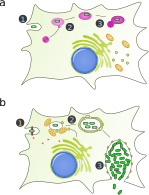
\includegraphics[width=\textwidth]{Parts/Part01/gfx/legionella_life_cycle.pdf}
    \caption[Infection by \textit{Legionella}.]{Infection by \textit{Legionella}: \textbf{a} Non infectious bacteria (green) are phagocytized by amoebae or macrophages (1), the early and late endosomes (pink) acidify the compartment (2), and it finally merges with the lysozome (3) where the bacteria is degraded. \textbf{b} Upon phagocytosis, \textit{Legionella} uses its type IV secretion system to secrete effector proteins (red triangles) into the cytoplasm and evades the endosome route (1). Instead, it stays in a "\textit{Legionella} containing vesicle" (LCV) and recruits mitochondria (orange) and endoplasmic reticulum-derived vescicles (yellow) (2). The bacteria keeps replicating in the LCV until it bursts out and infects other cells.}
	\label{fig:01-01:legionella}
\end{figure}

\subsection{Life cycle}
\textit{L. pneumophila} follows a biphasic life cycle. It can survive in the extracellular environment and thrives in fresh water. It can either spread planktonically as a free living organism using its flagella to reach new hosts, or by associating with biofilms \citep{hilbiLegionellaSppOutdoors2011,steinertLegionellaPneumophilaAquatic2002}. This extracellular phase is called the "transmissive form", as bacteria will search for new host cells but will not replicate \cite{byrneExpressionLegionellaPneumophilaVirulence1998}. In contrast, when entering a host cell, the bacterium enters the "replicative form". In that stage, the  bacterium takes advantage of the abundant resources and nutrient available in the host cell to replicate as much as possible.

Switching between replicative and transmissive phases requires consequent morphogenetic and metabolic changes, mobilizing expression changes in almost half of the known genes \cite{steinertLegionellaPneumophilaAquatic2002}. Low nutrient and high stress conditions cause \textit{L. pneumophila} to enter transmissive phase, activating genes related to motility and virulence, such as its type IV secretion system. When entering the replicative phase, genes related to sugar and gluconate uptake and amino-acid catabolism are upregulated instead. The bacteria become acid resistant and replicate in the \acrshort{LCV} until the nutrient pool is depleted.

Comparison of gene expression profiles between \textit{L. pneumophila} grown \textit{in vitro} in the absence of host, and \textit{in vivo} in the amoeba \textit{A. castellanii} revealed that changes associated with progression from exponential growth to stationary phase are similar to those observed between replicative and transmissive phases \cite{bruggemannVirulenceStrategiesInfecting2006}. In \textit{in vitro} cultures, stationary phase refers to the time when bacteria stop replicating for lack of nutrients. This suggests that the biphasic life cycle of \textit{L. pneumophila} is governed mostly by nutrients present in the environment \cite{olivaLifeCyclePneumophila2018}.

The master regulator underlying this switch is thought to be the carbon storage regulator protein A (CsrA). CsrA is an RNA binding protein with over 400 target transcripts identified, including 40 effector proteins and genes related to virulence and motility. In replicative phase, CsrA binds its target transcripts to repress their translation. When nutrients are running low, \textit{L. pneumophila} produces the alarmone (p)ppGpp, which triggers the expression of noncoding transcripts with strong affinity for CsrA. This prevents CsrA from binding its targets and enables the translation of virulence genes \cite{sahrLegionellaPneumophilaGenome2017}.

\subsection{Host interactions}

While inside the host, \textit{L. pneumophila} consumes products from the host cell for energy production. It relies mainly on serine, threonine and other amino acids but can also scavenge carbohydrates such as gluconate \cite{bruggemannVirulenceStrategiesInfecting2006}. Those nutrients are transferred from the host cytoplasm to the LCV by transporters on the LCV membrane \cite{wielandIntracellularMultiplicationLegionella2005}. The bacterium can increase the availability of nutrients in the host cell using its effector proteins. One example is the AnkB effector which can poly-ubiquitinate host proteins, causing their degradation by the host proteasome, resulting in amino acids which can then be imported into the LCV and consumed \cite{priceMolecularMimicryFBox2009}. Other effectors block host protein translation to increase the pool of free amino acid available for consumption by \textit{L. pneumophila} \cite{deleonPositiveNegativeRegulation2017}.

The host trafficking system is also hijacked, resulting in the recruitment mitochondria and \acrfull{ER} membrane vesicles to the LCV. This is likely achieved by modulating the activity of host GTPases, such as Arf1, Sar1 and Rab1 \cite{isbergLegionellaPneumophilaReplication2009}. Some \textit{Legionella} effectors directly affect the host actin cytoskeleton, which is important in many cellular processes including vesicle trafficking \citep{liuLegionellaEffectorDisrupts2017,francoLegionellaPneumophilaEffector2012}.

\textit{L. pneumophila} also ensures successful infection by promoting host cell survival. The effector SdhA interferes with host cell apoptosis by inhibiting caspases \cite{lagunaLegionellaPneumophilatranslocatedSubstrate2006}. All these interference with the host cell signalling pathways are likely bound to affect its expression program. It was recently found that one of the effectors secreted by \textit{L. pneumophila} directly affects the host epigenetic state. This effector, named RomA, is a histone methyltransferase which can alter the histone methylation state throughout the host genome and affects the expression of a large number of genes \cite{rolandoLegionellaPneumophilaEffector2013}.

There is still much to learn about the interaction between \textit{Legionella} effectors and its host regulation, but that the bacteria is able to modify directly nucleosomes of the host unveiled a new level of intimacy between bacterial endosymbionts and their host, with fascinating perspectives. Besides, epigenetics and gene expression are tightly connected with spatial genome organization in eukaryotes \cite{dixonChromatinDomainsUnit2016,schneiderDynamicsInterplayNuclear2007}, providing a new angle to approach the study of host-pathogen interactions.

\section{\textit{Salmonella enterica}}

Unlike \textit{L. pneumophila}, \textit{S. enterica} infects not only mammals but also birds and reptiles \cite{uzzauHostAdaptedSerotypes2000}. It is also a model for intracellular bacterial infections and a major human pathogen. \textit{Salmonella} is a facultative intracellular parasite which can infect macrophages, dendritic, epithelial and microfold (M) cells. It is usually transmitted by ingestion of contaminated food and colonizes the gastrointestinal tract. \textit{Salmonella} isolates are classified into 2,500 serovars based on their lipopolysaccharides and flagellar antigens. While most serovars, referred to as "non-typhoidal" cause salmonellosis, a self-limiting enteritis, "typhoidal" serovars are human restricted and cause a systemic disease known as typhoid fever \cite{larockSalmonellaeInteractionsHost2015}.

Every year, it is estimated that there are 16.6 million cases of typhoid fever causing 600,000 deaths in the world, and 1.3 billion cases of acute gastroenteritis associated with \textit{Salmonella}, responsible for 3 million deaths \cite{pangTyphoidFeverOther1995}. Most of the current knowledge on \textit{Salmonella} infection biology was built on the non-typhoidal serovar \textit{S. enterica} subsp. \textit{enterica} serovar Typhimurium \cite{larockSalmonellaeInteractionsHost2015}. 

Much like \textit{Legionella}, when \textit{Salmonella} enters the host cell, it is engulfed into a \acrfull{SCV}  and secretes effector proteins into the host cytoplasm. This is done via two independent type 3 secretion systems (T3SS) named SPI1 and SPI2. These two systems are encoded by and named after the \textit{Salmonella pathogenicity island}, which \textit{Salmonella} likely acquired through horizontal gene transfer.

The mechanisms employed by \textit{Salmonella} to infect host cells are similar to \textit{Legionella}. For example, they encode effectors that also activate the host gene Arf1 to promote bacterial uptake and actin polymerization \cite{larockSalmonellaeInteractionsHost2015}. Although no effector of \textit{Salmonella} is known to directly affect the host epigenetic state, a global rewriting of histone modifications and DNA methylation \cite{szteinSalmonellaEntericaSerovar2020,wangChickenCecalDNA2020} is observed in \textit{Salmonella}-infected cells. Furthermore, histone modifications was associated with susceptibility to Salmonella infection in chickens \cite{gouEpigeneticModificationTLRs2012}, further highlighting the importance of investigating chromatin changes during bacterial infection.


 % Chapter 1
% Chapter X

\chapter{Infection through the lense of genomics} % Chapter title

\label{ch:01-02} % For referencing the chapter elsewhere, use \autoref{ch:name} 

%----------------------------------------------------------------------------------------

The toolset to detect and investigate bacterial infection traditionally included biochemical assays and microscopy. The recent technological advances in DNA sequencing have spurred a rapid extension of this toolset with NGS-derived methods. Here we introduce the different ways genomics to provide biological insights into the biology of bacterial pathogens.

\section{Pathogen characterization}

The most fundamental task related to infection in biomedical research is to detect the presence of infectious agents and identify their nature. This allows to test patients presenting suspicious symptoms for the presence of known pathogens, or determine the pathogenicity of a particular strain. 

This is traditionally achieved using molecular biology techniques.

\section{Genomics to probe homeostasis}

When host cells are exposed to or infected by a pathogen, their homeostatic state will be disrupted. This disruption is a combiantion of host-triggered reactions to improve its survival, and alterations caused by the pathogen to colonize the host cell. Untangling these two phenomenon is a complex issue in itself, but investigating what biological functions or pathways are disrupted upon infection can already give good  pointers to important players in the infeciton.

Multiple levels of regulation are affected, from gene expression to epigenetic states, and over the years, a vast arsenal of NGS techniques have been developed to read thse regulatory states. For example, ChIPseq, ...

he transcribed genes, present in the cell in the form of RNA, can also be read using the same DNA sequencing technologies. This allows one to estimate the expression of genes from the amount of RNA present in the cells. This is useful when studying infection, as the expression of each gene can be compared between uninfected and infected cells to detect which biological functions are perturbed.



\section{Capturing chromosome conformation}

The use of genomics to investigate the three-dimensional organisation of the genome started with the invention of \acrfull{3C} \cite{Dekker2002}. This technique allowed to measure the frequency of physical interactions a pair of loci. This is done by crosslinking the genome with formaldehyde, which forms stable bonds between DNA and proteins, and subsequently digesting the genome with a restriction enzyme. The digested genome is then relilgated, and the religation will happen with different neighbouring fragment. Loci which are closer in space will be religated more often with each other in the population of cells. The crosslink is then reverted and qPCR is used to measure the quantity of religated products containing the two loci of interest. 

Since then, many derivative of the \acrshort{3C} technique have been developed. The most significant improvement was brought by Hi-C. This method works similarly to 3C except that next generation sequencing is used instead of qPCR. This allows to quantify the interaction frequency of all versus all loci in the genome instead of using specific primers for a pair of locus. Hi-C also has an additional step where biotinylated bases are added during religation. This allows to pull-down religation products using streptavidin so that only products that underwent the digestion-religation process are sequenced.

Hi-C allows to generate interaction frequency maps of the whole genome wich reflect its 3D structure.

\section{Combining layers of biological informations}

\section{Reproducibility and reliability challenges}
% Impact of the reproducibility crisis
% Software quality
% The importance of standardisation
 % Chapter 2
% Chapter X

\chapter{The importance of genome assembly} % Chapter title

\label{ch:01-03} % For referencing the chapter elsewhere, use \autoref{ch:name} 

%----------------------------------------------------------------------------------------
Most of the genomic techniques presented before require a complete reference genome as downstream analyses will rely on the relative position of different biological elements on the genome sequence to draw biological conclusions. 

A good phylogenetic representation of sequenced genomes is also crucial for comparative analyses. This allows for example to  identify recent \acrshort{HGT} events. Here we describe in more detail the process of genome assembly and its relevance to infection genomics.

\section{From contigs to chromosomes}
% Define terminology, explain advantages of chromosome level assemblies and how to generate them
% Subsections for bionano, linked reads and Hi-C
% Maybe a quick mention of haplotype-resolved assemblies and genome-graphs

Genome assembly consists in reconstructing the linear sequence of the genome from the readings of DNA sequencing technologies. Although the final assembly depends on the quality of these readings, the algorithms used to combine their information are also crucial.

In the early days of genome sequencing, the Sanger method was used to read DNA sequences \cite{sangerDNASequencingChainterminating1977}. Sanger is a low throughput, but highly accurate sequencing method. This technology allowed to unveil the complete genome sequences of viruses \citep{sangerNucleotideSequenceBacteriophage1982,baerDNASequenceExpression1984} and the yeast genome \cite{oliverCompleteDNASequence1992}. A common practice at the time, was to clone a small genomic region of \textasciitilde 10kb into a plasmid, and fragment it \cite{thierryCompleteSequenceKb1990}. The resulting fragments were sequenced and the sequencing readout, in the form of gels, had to be deciphered by scientists, one nucleotide at a time. The cloned region was then assembled manually by searching for overlaps between fragments.

Further technological improvements allowed to automate the sequencing process to tackle the sequencing of larger eukaryotic genomes. Early genome sequencing projects were performed using laborious and costly experimental methods, such as \acrfull{BAC}, which involved cloning long overlapping pieces of DNA of the genome into bacteria. These pieces were then experimentally amplified and sequenced in parallel. Ovelapping ends from each of those sequences had to be aligned to recover the entire chromosome sequence. The first genome sequencing projects were sizable undertakings requiring the collaboration of many research groups throughout the world \citep{collinsNewFiveyearPlan1993,adamsGenomeSequenceDrosophila2000,oliverCompleteDNASequence1992}, but technological advancements progressively reduced the cost and time required. A decisive change was the development of shotgun sequencing \cite{venterSequenceHumanGenome2001}, which involves randomly sequencing regions to cover the entire genome.

With the advent of \acrfull{NGS}, shotgun sequencing became the standard for whole genome sequencing. \acrshort{NGS} has much higher throughput than Sanger sequencing, allowing to sequence megabases of DNA very quickly. However, it can only read short sequences at a time, referred to as \Gls{read}s. Classic overlap-based genome assembly algorithms used in previous sequencing projects could not scale to such large numbers of short reads. This called for the development of more efficient genome assembly algorithms.

The goal of an assembler is to generate a highly contiguous genome sequence from a large number of short reads. Early algorithms computed pairwise alignments between all reads to build an overlap graph (Fig. \ref{fig:01-03:debruijn}a). The genome could then be assembled by finding th e Hamiltonian path of the graph, which passes once through every node. However, finding this approach is computationally expensive and cannot be used with high sequencing throughput \cite{compeauHowApplyBruijn2011}. This lead to the development of de Bruijn-based assembly algorithms, which many most modern still use \citep{simpsonABySSParallelAssembler2009,zerbinoVelvetAlgorithmsNovo2008}. de Bruijn assemblers split reads into short \Gls{k-mer}s which they use to generate a de Bruijn graph. In these graphs, k-mer sequences represent edges, and the overlap between adjacent k-mers within reads are the nodes (Fig. \ref{fig:01-03:debruijn}b). To assemble a genome, assemblers need to find the Eulerian path, which passes through every edge once. However this is often not possible because of repeated sequences in the genome, sequencing errors and haplotypes \cite{simpsonTheoryPracticeGenome2015}. Whenever a repeated sequence is longer than the read itself, the graph can not be solved and heuristics have to be used. Rather than a single fully resolved genome, the resulting assemblies usually have a relatively high number of independent pieces called \Gls{contig}s.

\begin{figure}
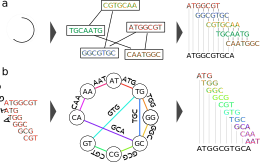
\includegraphics[width=\textwidth]{Parts/Part01/gfx/debruijn.pdf}
\caption[Graphs in genome assembly.]{Graphs in genome assembly: A small circular genome is sequenced and the resulting reads are shown in color \textbf{a}: Early assembling techniques computed all pairwise alignments between reads to represent them as nodes in an overlap graph and their overlaps as edges. The genome sequence can be retrieved by finding a path going through each read exactly once. \textbf{b}: Modern assemblers first split reads into their constituent k-mers and represent the k-mers as edges in a de Bruijn graph where nodes are the k-1 overlap between two k-mers located in the same read. The path going through each edge once is computed to solve the graph. K-mers are extracted from the edges visited to retrieve the genome sequence. Adapted from \cite{compeauHowApplyBruijn2011}}
\label{fig:01-03:debruijn}
\end{figure}

Third generation sequencing partially alleviates this issue by generating long albeit less accurate reads. Read lengths up to hundreds of thousands of basepairs can be generated, which allows to span most repeated regions. Recently, these technologies were used to generate telomere-to-telomere assemblies of several human chromosomes \citep{migaTelomeretotelomereAssemblyComplete2020,logsdonStructureFunctionEvolution2021}. Third generation sequencing techniques still suffer from their lower base calling accuracy resulting in assemblies with high point error rates (>10\%) and indels \cite{weiratherComprehensiveComparisonPacific2017,jainNanoporeSequencingAssembly2018}. To remove these errors, some methods have been developed to correct long reads before assembly, either by correcting long reads among themselves \cite{morisseScalableLongRead2021}, or using a separate set of short accurate reads to erase sequencing errors in long reads \cite{wangFMLRCHybridLong2018}. Most long reads correction tools are also unable to differentiate between SNPs and sequencing errors, which result in the loss of haplotype information and prevents the generation of haplotype-resolved assemblies. Some long read correction methods have recently been developed to preserve haplotypes information \cite{holleyRatatoskHybridError2021}. One major drawback of read correction methods is their high computational cost, as they require to align high number of reads to each others. An alternative strategy is to use the uncorrected reads to assemble the genome and perform errror correction directly on the assembly, a process known as \Gls{polishing}. Traditional short read polishers work by aligning short reads to the assembly and replacing each position of the assembly by the consensus of short reads \cite{vaserFastAccurateNovo2017}. Additionally, they can correct larger scale misassemblies such as indels by using the pair-end information and alignment discrepancies \cite{walkerPilonIntegratedTool2014}. Some polishers have obtained better polishing accuracy by combining the information in short and long reads \cite{kunduHyPoSuperFast2019}.

More recently the emergence of specialized technologies aimed at scaffolding have allowed to generate even more continuous and correct genomes at reduced costs. One example is the recent rebirth of optical mapping to introduce fluorescent probes into chromosomes at specific sites \cite{lamGenomeMappingNanochannel2012}. The order of these probes and their relative distance form barcodes which can then be used to scaffold genome assemblies, reorder and merge contigs. This is often combined with Hi-C to generate highly continuous assemblies even in the presence of repeated sequences.

A growing number of genome assemblies combine several of these different technologies to bring the number of scaffolds as close as possible to the real number of chromosomes (Fig. \ref{fig:01-03:assembly}).

\begin{figure}[htb]
    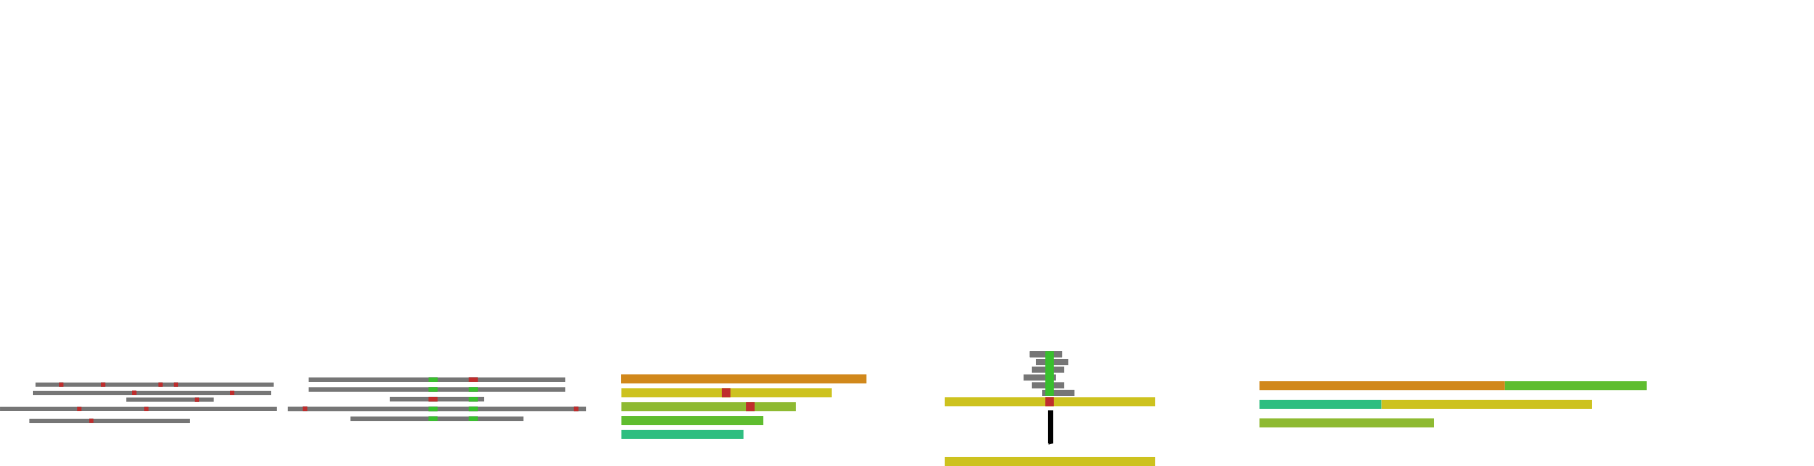
\includegraphics[width=\textwidth]{Parts/Part01/gfx/assembly_pipeline.pdf}
    \caption[Example of a third generation sequencing assembly pipeline.]{Example of a typical assembly pipeline using third generation sequencing. The error prone long reads are first corrected by pairwise comparisons. The corrected reads are assembled into contigs using their overlaps. The remaining sequencing errors in the assembly are removed by polishing with accurate short reads. Other sources of information can then be used to combine contigs into scaffolds.}
    \label{fig:01-03:assembly}
\end{figure}

\section{Phylogenetic representation}
% HGT detection requires a reference group

A common way to analyze the genome of new microorganisms is to compare it to other species. To achieve this, one needs to have other closely related genomes available. A common case where dense species genome representation is required is when attempting to detect \acrshort{HGT}.

\acrshort{HGT} detection methods often rely on discordance between gene trees and species trees. A horizontally transferred gene between two distant species would show strong sequence similarity \cite{ravenhallInferringHorizontalGene2015}. For this reason, detection of recent events requires genomes of closely related organisms as a comparison point.

\begin{figure}[htb]
    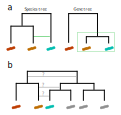
\includegraphics[width=\textwidth]{Parts/Part01/gfx/phylo_hgt.pdf}
    \caption[Phylogenetic representation of an HGT event.]{Phylogenetic representation of an HGT event. \textbf{a:} An HGT event between two species (shown with a green arrow) can be detected through discrepencies between the species (left) and gene (right) trees. \textbf{b:} In cases where genomes of closely related species are unavailable (greyed out organisms), the origin of the horizontal transfer cannot be accurately inferred (possible events shown with grey arrows).}
    \label{fig:01-03:phylo-hgt}
\end{figure}

Another frequent analysis when comparing a group of strains or species of microorganisms is to define the common set of genes they share, known as pangenome. This also allows the identification of genes specific to a particular genome, known as accessory genome. Such sets can be helpful to determine metabolic reactions associated with species or niches, however they heavily depend on the proportion of available species in the group.

Lately, several large consortia \citep{genome10kcommunityofscientistsGenome10KProposal2009,poelchauI5kWorkspaceNAL2015,DarwinTreeLife} undertook the daunting task of sequencing thousands of organisms throughout the tree of life. For the aforementioned reasons, these large collaborations are likely to greatly improve the power of comparative genomic analyses results in the future.

\section{The transition to genome graphs}

Until recently, all reference genomes were exclusively stored as linear (or circular) sequences of DNA. This linear sequence is often obtained from a mix of multiple individuals, or alleles within an individual. It is effectively a semi-arbitrary combination of multiple haplotypes collapsed into an artificial consensus sequence. A more accurate alternative is to produce a reference sequence graph instead \cite{churchExtendingReferenceAssembly2015}. Given a collection of haplotypes, individuals, or strains of a species, one can generate a graph where identical regions are collapsed, while sample-specific variants form bubbles retaining the genetic variability. As this approach is relatively recent, few algorithms have been developed to operate on sequence graphs, making their applications very limited.

The shift to genome graphs is promising for the analysis of bacterial samples, where alignment can be performed on multiple strain references at the same time. Doing this with a collection of linear genome incurs mapping bias due to ambiguous alignments between redundant regions between references \cite{liDesignConstructionReference2020}. Similarly, genome graphs also allow systematic alignment to different alleles in polyploid organisms, solving the issue of allele-specific mapping bias in linear references \cite{vandegeijnWASPAllelespecificSoftware2015}.  % Chapter 3
%% Chapter X

\chapter{Thesis objectives} % Chapter title

\label{ch:01-04} % For referencing the chapter elsewhere, use \autoref{ch:name} 

Throughout this first part, we have laid out the scope of host-pathogen interactions and summarized the current state of genomics in relation to regulation and 3D genomes. Although genomics is a fast changing field, there is a need for computational tools to extract meaningful biological information from the wealth of data.

Throughout the next part, we will introduce our contributions to the field and main results. In the first chapter, we explain our methodological developments related to chromosome conformation capture technologies. In the second chapter, we will present our chromosome scale genome assembly of \textit{A. castellanii}. We then use this resource for our main findings on the genomic changes happening during infection by \textit{L. pneumophila}. Chapter 3 will focus on murine bone macrophages infection by \textit{S. enterica} and the genomic alterations it entails. Finally, in chapter 4, we will discuss additional results related to the implications of viral integrations linked to hepatocellular carcinoma in the human genome. We will end with part 3 where we discuss various aspects of genomics in infection biology, including prospects and limitations.

In this work, we develop accessible and performant methods to extract information from 3C technologies and use them to identify changes happening during infections in various organisms. We then use external data such as gene expression to assess the genes involved in those alterations and discuss how they could be associated with the infection process.
%----------------------------------------------------------------------------------------

 % Chapter 4 
